\section{Current TP8 native-AR results}
\label{sec:current-native}

The primary result is the September 13--14 fresh-process revalidation on the
merged original-V4 implementation, archived at \commit{3d73a75923}. All seven
native graph tiers were captured and observed with matching active input and
executed rows during full residency. The model remained a single TP8/EP1
instance. No DSpark, MTP, or approximate routed-expert verification contributed
to the following table.

\begin{table}[htbp]
  \centering
  \caption{Formal native P/D matrix: P and resident D are three-round medians;
  HTTP aggregates complete measured waves. Prefill divides aggregate input by
  wave time to the last first token. Resident and HTTP decode are distinct metrics.}
  \label{tab:tp8-matrix}
  % Generated from data/results.json by prepare_report_data.py.
\begin{tabular}{@{}rrrr@{}}
\toprule
C & Prefill input tok/s & Resident output tok/s & HTTP output tok/s \\
\midrule
1 & 4676.39 & 87.60 & 86.39 \\
2 & 4989.25 & 109.94 & 102.41 \\
4 & 5265.43 & 188.71 & 148.50 \\
8 & 5099.23 & 334.18 & 254.45 \\
16 & 5171.36 & 608.23 & 422.51 \\
32 & 5254.98 & 1044.32 & 680.61 \\
64 & 5250.05 & 1334.24 & 848.14 \\
\bottomrule
\end{tabular}

\end{table}

\begin{figure}[htbp]
  \centering
  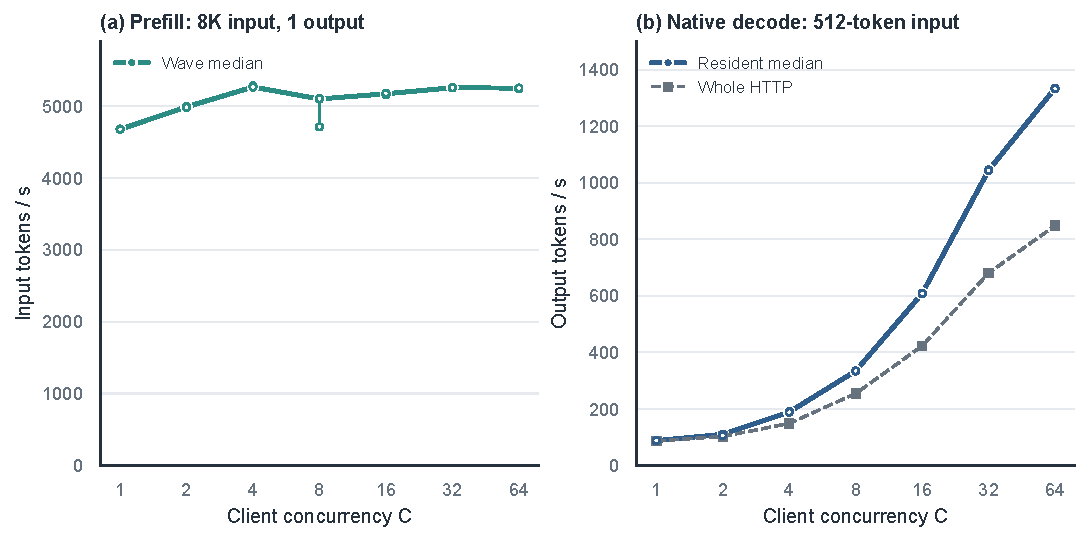
\includegraphics[width=\textwidth]{figures/tp8_pd_matrix.pdf}
  \caption{Latest TP8 matrix. Colored points/lines show three-round medians;
  thin vertical ranges and small points are actual rounds, not confidence
  intervals. Gray decode points are complete-wave HTTP rates, not a slower
  kernel configuration. Concurrency uses a base-2 axis.}
  \label{fig:tp8-pd}
\end{figure}

\paragraph{Protocol boundaries.}
Prefill uses 8191--8192-token public-source prompts, fresh cache salts, and one
output token. At C64 the wave contains about 524k input tokens, admitted at
most 16 requests at a time with a 36,864-token chunk budget. C64 therefore does
not mean one M64 prefill kernel or 64 simultaneous large prefill requests.
Decode uses 511--512-token inputs, greedy sampling, natural EOS, and at most
2048 output tokens. Each formal round accumulates at least 30 s of common
resident windows; explicit warmups are excluded. The 64-case corpus extends
the earlier 32-case public-source corpus without changing those first 32 cases.
Duration-dependent wave counts can expose different case mixtures, which are
preserved in raw records.

\paragraph{C1 supplement.}
The seven-tier run originally omitted the existing C1-only wo\_a GEMV opt-in.
It was restored, independently tested, and measured for three new C1 rounds.
The C1 row above uses that supplement. C2--64 resident windows cannot select
the M1 kernel; their whole-wave HTTP numbers nevertheless retain the measured
GEMV-off drain behavior. We do not claim a newly measured all-on HTTP matrix.

\paragraph{Interpretation.}
Prefill plateaus near 5.2k aggregate input tok/s under this admission/chunk
policy. Decode continues scaling through C64, reaching 1334.24 resident output
tok/s, but complete-wave throughput is 848.14 tok/s. The gap includes admission,
prefill, uneven answer lengths, and drain. It is not a measured host-only
overhead term. The C8 prefill rounds include 4710.94 alongside approximately
5100 input tok/s; this slower measured round is retained, not silently trimmed.
No matched current TP4 seven-tier matrix is available in the retained evidence,
so a TP4-to-TP8 scaling factor is not reported.

\subsection{Empty C4 tiles: pool capacity is not active context}

With a 1M logical pool, the C4 logits launch could cover 262,144 key positions
even when only a short prefix was active. Beyond the raw-token threshold near
2048, many launched tiles had no valid keys but still performed unnecessary
query loading and dot work. The exact native-decode guard skips this empty
work while retaining defined zero stores, unchanged active computation,
sequence lengths, Top-K semantics, and physical index mapping.

Seven component shapes, 100 mutations per shape, and 1000 graph replays per
shape checked score bits and logical/physical indices. Fully populated control
cases did not exhibit the empty-work benefit. At M32, the diagnostic component
dropped from approximately 6934 to 837 microseconds; this is not a whole-model
speed prediction.

A separate matched 8K-input C32 service ABBA measured
169.657 / 611.103 / 610.853 / 169.843 resident output tok/s, a 3.599-fold
candidate/control ratio. Complete HTTP rates were approximately 83.18 / 128.85 /
128.88 / 83.26 tok/s. The different ratios illustrate why the measurement
boundary must be explicit. This 8K test is not the 512-input formal decode
table, and its multiplier must not be applied to that table. This fix is
native-decode scoped; the earlier prefill trivial-row skip is a different path.

\subsection{Recovering the existing C1 projection specialization}

The restored wave64 wo\_a GEMV measured 30.75$\rightarrow$6.88 microseconds in
its component test. All 100 tested mutations were finite and repeatable, but
only 70 were bit-equal to the former einsum path; the maximum relative L2
error against a float32 reference was about 0.00179 on the test inputs.
It retains checkpoint weights while changing floating reduction.

The service ABBA was 79.558 / 87.583 / 87.504 / 79.151 resident output tok/s:
+10.32\% by mean candidate/control arms. Candidate repeats had identical
completion sequences in that test, and France passed. The separate formal C1
median is 87.599. These controls are more informative than an unpaired
comparison with the August 74.5 HTTP result.

\begin{figure}[htbp]
  \centering
  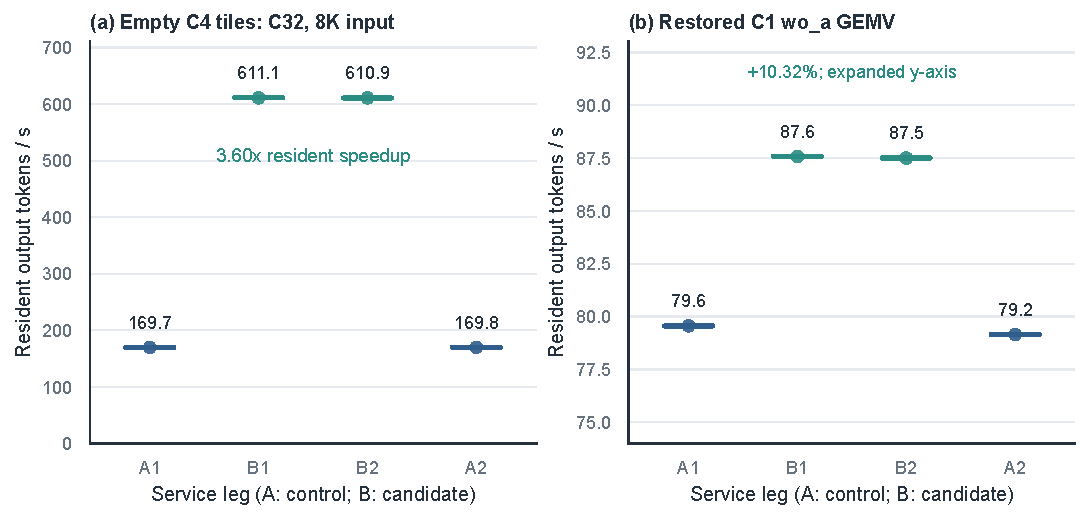
\includegraphics[width=\textwidth]{figures/native_abba.pdf}
  \caption{Separate native ABBA experiments: empty C4 tiles at C32 with 8K
  inputs, and the C1 projection specialization with 512-token code inputs.
  The right axis is expanded; the experiments must not be multiplied together.}
  \label{fig:native-abba}
\end{figure}

\subsection{Down-consumer pilot: a small C32 gain, no C1 kernel change}

The follow-up at \commit{fb2e39fca9} replaces the M32 second quantization/down
chain with a CTA16 consumer. Each CTA reads the already-rounded BF16
intermediate, forms group32 INT8 values/scales in LDS, computes its output
stripe, and retains the existing FP32 top-k partial and fixed reduction.
The current gate, sorter, original weights, attention, and TP collectives are
unchanged. The selector is limited to native TP8/EP1, M32/I256 and A4/R2
geometry; it remains default-off.

On one GCD, synthetic diverse/skewed inputs reduced quant+down+reduction from
130.542 to 115.907 microseconds and 81.615 to 70.791 microseconds, respectively.
Each distribution passed 100 mutations of inputs, routes, weights and scales
and 1000 checked graph replays. Comparisons used numeric element equality,
not a signed-zero-bit check. This is neither the full routed stage nor a
captured real-layer oracle.

The service screen uses two natural-EOS waves per leg with the same 32 code
requests, rather than the duration-driven formal 64-case protocol. C32 leg
medians are 1047.763 / 1060.206 / 1061.203 / 1041.459 resident tok/s. Mean
control 1044.611 versus candidate 1060.705 gives +1.541\%; the return control
changes $-0.602\%$, and candidate legs differ 0.094\%. Every candidate wave
exceeds every control wave. Whole HTTP rates vary with answer length and do
not establish the same percentage gain.

The conditional C1 test is an isolation check, not an M1 port: the existing
direct M1 down kernel already quantizes in LDS, with a different rounding
contract. Its control/candidate means are 89.722/90.024 tok/s; the 0.34\%
variation is not attributed to an unselected kernel. All eight 1453-token C1
completions match across arms. This fixed-case screen does not supersede the
formal multi-case C1 value. For C32, control outputs themselves vary across
waves; neither whole-model bitwise parity nor code-answer factual correctness
is established. All 264 measured pilot responses passed independent ID/text
integrity checks, and all service France sentinels passed.

\begin{figure}[htbp]
  \centering
  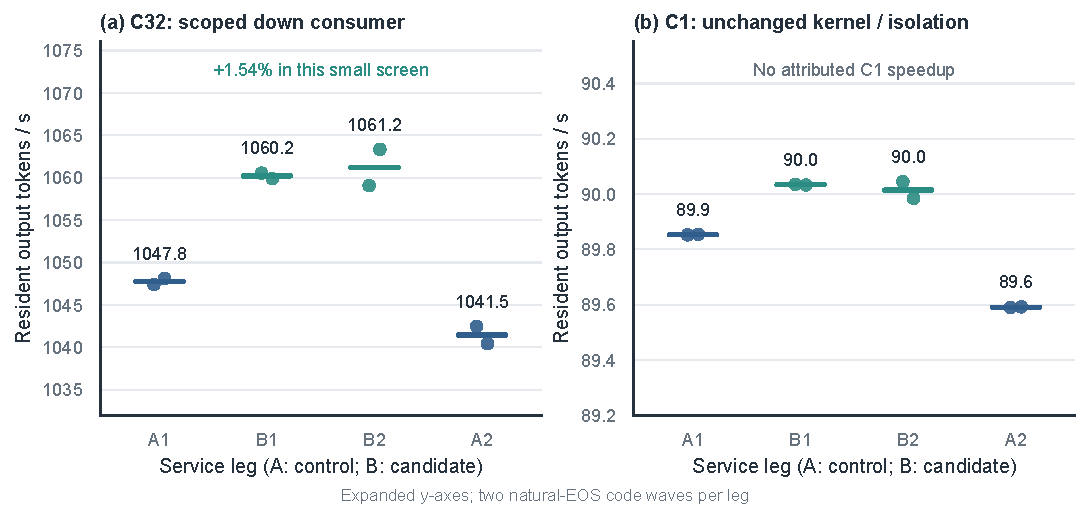
\includegraphics[width=\textwidth]{figures/down_consumer_abba.pdf}
  \caption{Default-off down-consumer pilot, expanded y-axes. Dots are the two
  measured waves per leg; short bars mark their median. C1 never executes
  the candidate and is a negative-control scope check.}
  \label{fig:consumer-abba}
\end{figure}
